% !TEX encoding = UTF-8
% !LW recipe = XeLaTeX (软件学报 rjthesis)
% 《软件学报》排版稿 — 基于 docs/latex-models/software-journal/rjthesis.cls
% 编译：./scripts/build_pdf_jos.sh
% 使用系统 Noto CJK 字体，避免 IDE/TeX Live 下 Fandol 的 Script=CJK 警告
\PassOptionsToClass{fontset=ubuntu,twoside,UTF8}{ctexart}
\documentclass{rjthesis}
% ubuntu 字体集无 \fangsong/\lishu，rjthesis 标题区会用到
\providecommand{\fangsong}{\kaishu}
\providecommand{\lishu}{\songti}
\usepackage{graphicx}
\graphicspath{{../figures/}}
\usepackage{amsmath}
\usepackage{booktabs}
\usepackage[super,square,sort&compress]{natbib}
\usepackage{hyperref}
\usepackage{bookmark}
\hypersetup{colorlinks=true,linkcolor=blue,citecolor=blue,urlcolor=blue}
\usepackage[ruled,vlined,linesnumbered]{algorithm2e}
\providecommand{\kai}{\kaishu}

% ---------- 元数据 ----------
\rjhead{石\hspace{1em}洪\hspace{1em}雷\hspace{1em}等:分布式定向日志采集组件}
\fancyhead[RE]{\xiaowuhao\textit{\xiaowuhao Journal of Software} {\kai 软件学报}}

\rjtitle{微服务架构下分布式定向日志采集组件的设计与实现}
\rjauthor{石\hspace{1em}洪\hspace{1em}雷, 赵\hspace{1em}涓\hspace{1em}涓}
\rjinfor{（太原理工大学，山西 太原  030024）\\
通讯作者: 石洪雷, E-mail: shihonglei0042@link.tyut.edu.cn
}

\begin{document}

\rjmaketitle

% 摘要与关键词（共享内容，供 main-zh.tex 和 main-jos.tex 引用）
% 修改摘要只需编辑此文件，两个入口文件自动同步。

% ========== 中文摘要 ==========
\newcommand{\AbstractContentZh}{%
微服务架构下，日志来源高度分散、格式各异、总量庞大，给节点资源、网络带宽和集中存储都带来了很大压力。本文提出一种分布式定向日志采集框架与原型组件，核心思路是``只采必要日志''。框架分为三层：网关预筛选、节点定向采集和中心二次过滤。日志中心根据网关流量日志动态生成关注清单，驱动各节点按清单定向采集应用日志。节点侧采用固定缓存块算法和压力感知指数退避机制，在资源受限时保障传输可靠性。三层之间通过定向策略三次转换算法保持策略语义一致。原型基于 Go 语言和 Grafana Loki 实现，应用日志采用 Apache Combined 风格并与网关 URL 对齐。实验在 WSL/Docker 八节点集群上进行对比测试（180\,s、并发 50、每模式重复 3 次），并补充了十六/三十二节点规模复核、策略仿真消融、基于真实分布的多进程模拟与算法微基准测试。结果显示，定向采集将 Loki 入库量控制在 72 条，而同架构全量基线为 4388$\pm$1 条，降幅达 98.4\%（该降幅包含定向过滤与发射频率差异的联合效果；多进程同频模拟表明策略过滤的独立降幅为 67.8\%）。清空统计后的规模复核中，十六节点 Loki 入库为 48.0$\pm$5.2 条/轮，三十二节点稳定在 99.0$\pm$0.0 条/轮。Agent 平均 CPU 与内存分别降低 37.5\% 和 2.0\%（绝对值均较低）。端到端链路（Nginx 共享内存 $\rightarrow$ Agent gRPC $\rightarrow$ Redis $\rightarrow$ 关注清单生成）已实测打通。关注清单生成算法在 5000 条日志上耗时约 15\,ms，指数退避机制通过 \texttt{agent/pkg/retry/backoff\_test.go} 全部单元测试。%
}

% ========== 英文摘要 ==========
\newcommand{\AbstractContentEn}{%
Microservice architectures scatter log sources across many independently deployed services, each emitting logs in heterogeneous formats whose aggregate volume grows linearly with request concurrency. The resulting overhead on node CPU, network bandwidth, and centralized storage motivates a shift from full-volume collection to selective, traffic-aware ingestion. This paper proposes a distributed directed log collection framework whose guiding principle is to ``collect only what matters.'' The framework comprises three layers: gateway pre-filtering, node-side directed collection, and center-side secondary filtering. A log center dynamically generates an attention list from gateway traffic logs (URLs, status codes, response latencies) and distributes it to each node, which then collects only the application logs matching the list. Fixed-size cache blocks and pressure-aware exponential backoff maintain transmission reliability under resource constraints, while a triple strategy transformation keeps policy semantics consistent across all three layers. A prototype built with Go and Grafana Loki is evaluated on a WSL/Docker cluster. In eight-node comparison experiments (180\,s, concurrency 50, three repeats per mode), directed collection reduces Loki-ingested logs to 72 entries versus 4388$\pm$1 for the same-architecture full-collection baseline (98.4\% reduction, combining directed filtering and emission-rate differences; a same-frequency multi-process simulation isolates a 67.8\% independent reduction from policy filtering alone). Scale validations after counter reset show 48.0$\pm$5.2 ingested entries per round at 16 nodes and a stable 99.0$\pm$0.0 at 32 nodes. Mean agent CPU and memory overhead decrease by 37.5\% and 2.0\%, respectively, with absolute values remaining below 0.1\%. The end-to-end pipeline, from Nginx shared memory through agent gRPC upload, Redis caching, to attention-list generation, is verified in cluster experiments. Attention-list generation completes in approximately 15\,ms on 5000 log entries, and the exponential backoff module passes all unit tests in \texttt{agent/pkg/retry/backoff\_test.go}. These results suggest that gateway-driven directed collection can substantially reduce log ingestion volume at the collection front end without modifying application code.%
}

% ========== 中文关键词 ==========
\newcommand{\KeywordsZh}{微服务;分布式日志采集;定向过滤;动态策略;指数退避;Grafana Loki}

% ========== 英文关键词 ==========
\newcommand{\KeywordsEn}{microservice; distributed directed log collection; attention list; dynamic policy; exponential backoff; Grafana Loki}


\begin{rjabstract}
\AbstractContentZh
\end{rjabstract}
\rjkeywords{\KeywordsZh}

\begin{flushleft}
\xiaowuhao
{\hei 建议引用格式:}\hspace{1em}{\kai 石洪雷, 赵涓涓. 微服务架构下分布式定向日志采集组件的设计与实现[J]. 软件学报投稿稿, 2026.}
\end{flushleft}

\begin{flushleft}
\xiaowuhao
{\hei Abstract:}\hspace{1em}{\kai
\AbstractContentEn
}

\vspace{0.6em}
{\hei Key words:}\hspace{1em}{\kai \KeywordsEn}
\end{flushleft}

% ---------- 正文（与计算机学报版共用章节源文件）----------
% !TEX root = ../../main-jos.tex
\section{引言}

微服务架构通过服务拆分提升了系统的可扩展性与开发敏捷性，容器编排、Sidecar 与服务治理模式进一步推动了云原生应用的大规模部署\cite{burns2016patterns,burns2016borg,jamshidi2018microservices,richardson2018microservices,feng2020microservice,wuhuayao2020microdev}。但这种架构也使日志产生源头高度分散：每个服务实例独立输出日志，格式因技术栈而异，总量随请求并发线性增长。传统可观测性方案多采用\textbf{全量采集}策略，在中小规模场景下尚可接受；当集群规模达到数十至数百节点时，全量采集将导致节点 CPU/内存持续占用、南北向带宽成为瓶颈、存储与索引成本急剧上升，且海量低价值日志淹没关键故障信息\cite{liao2016logs,limingshu2019logmgmt,he2020logsurvey,usman2022observability}。

现有研究集中在日志存储压缩、采样过滤、故障诊断与 eBPF 无侵入采集等方向，但较少从\textbf{网关流量感知}出发，动态驱动各服务节点的应用日志定向采集。包航宇等\cite{bao2023aiops}总结智能运维实践与标准化框架，贾统等\cite{jiatong2020logdiag}系统梳理基于日志的分布式软件系统故障诊断技术。本文将研究对象前移到\textbf{采集前端}：利用网关作为南北向流量入口所掌握的 URL、状态码、响应时延等结构化信号，在不侵入业务代码的前提下识别高价值请求，进而指导下游节点仅采集与异常、慢请求相关的应用日志，实现``只采必要日志''。

\textbf{本文凝练的科学问题是}：在不侵入业务代码、不改变微服务业务调用链的条件下，能否将网关层可观测到的流量异常信号转化为节点侧应用日志采集约束，使系统在保留异常、慢请求等高价值上下文的同时，显著降低日志入库量、节点资源开销与后端存储压力？围绕该问题，本文进一步拆解出四个可验证子问题：网关流量日志能否动态生成有效关注清单；关注清单能否跨网关、节点与中心三层保持语义一致；定向采集是否会引入不可接受的 Sidecar 资源开销；固定缓存块与压力感知退避能否支撑中心不可达或短时拥塞下的可靠传输。

\textbf{本文的科学假设包括}：（H1）网关访问日志中的 URL、状态码与响应时延能够作为应用日志价值的先验信号，足以生成覆盖异常与慢请求模式的动态关注清单；（H2）将该关注清单下发至节点侧 Sidecar 后，可在规则级保留关键请求上下文，并使 Loki 入库量相较同架构全量采集显著下降；（H3）通过网关预筛选、节点定向采集与中心二次过滤之间的三次策略转换，可以维持跨层策略语义一致，形成端到端采集闭环；（H4）固定缓存块与指数退避机制能够在低资源占用下提供有界重试与传输缓冲能力。后文实验部分以 RQ1--RQ4 对上述假设进行映射验证。

基于上述科学问题与假设，本文提出\textbf{分布式定向日志采集框架与原型组件}。框架由\textbf{网关预筛选、节点定向采集、中心二次过滤}三层组成，并通过三次策略转换保持跨层语义一致。相较 Promtail/Fluent Bit 全量推送后在存储端压缩的传统方案，本文在采集前端将 Loki 入库量控制在百条量级（八节点实测详见 §6.3），从源头降低网络与存储开销。主要贡献如下：

（1）提出可复用的三层分布式定向采集框架，支持网关节点与微服务节点以 Sidecar 方式部署，中心负责策略生成与二次过滤，节点负责本地匹配、缓存与可靠上传，补足 AIOps 数据链路中的采集前端减量环节。

（2）给出关注清单动态生成、固定缓存块、定向策略三次转换及压力感知指数退避的形式化描述与 Go 语言实现；关注清单生成复杂度：排序实现上界为 $O(N\log N)$，最小堆实现为 $O(N\log K)$（$K$ 为清单大小，$K \ll N$；见算法~\ref{alg:attention}）。

（3）构建基于 Docker Compose 的可复现原型与多进程模拟器，在八节点集群上完成 180\,s、$n{=}3$ 重复对比实验、算法微基准与系统级组件消融，并补充清空统计后的十六/三十二节点规模复核；八节点结果显示 Loki 入库 72 条 vs.\ 全量 4388$\pm$1 条（含定向过滤与发射频率差异的联合效果），多进程同频模拟证实策略过滤独立降幅为 67.8\%，十六/三十二节点复核进一步验证了定向模式在扩展规模下的低入库量与低 Agent CPU 开销。

本文第 2 节综述相关工作；第 3 节介绍系统总体设计；第 4 节阐述关键算法；第 5 节描述实现细节；第 6 节给出实验与分析；第 7 节总结全文。

\section{相关工作}

\subsection{集中式日志栈}
ELK/EFK 以 Elasticsearch 为核心，检索能力强但索引成本高。Grafana Loki 采用标签索引，配合 Promtail 或 Fluent Bit 做节点推送，默认策略为全量或基于日志级别的静态过滤\cite{loki2019,turnbull2014monitoring,beyer2016sre}。国内外日志管理综述均指出，大规模软件系统日志在采集、传输、存储、解析和查询阶段都会引入显著成本\cite{liao2016logs,limingshu2019logmgmt,he2020logsurvey,candido2021logmonitoring}。现有降低成本的方法主要包括日志压缩、日志模式挖掘、模板解析、云日志低成本存储和离线数据集构建，例如 LogZip、Loghub、云日志存储系统与面向多节点日志流的异常模式检测\cite{liu2019logzip,zhu2020loghub,wei2023cloudlogstorage,wang2020logflow}。这些工作对入库后的压缩、解析和数据治理具有价值，但多数默认日志已经被采集到中心端；本文关注的是日志进入中心前的\textbf{采集前端定向减量}。

\subsection{采样与追踪关联}
OpenTelemetry 尾部采样（Tail-based Sampling）依赖分布式追踪上下文，在请求完成后决定是否保留关联 span 或关联日志\cite{otel_tail}。工业调研和云原生可观测性综述显示，追踪、指标和日志三类遥测数据在微服务排障中通常需要联合分析\cite{li2021observability,kosinska2023observability,usman2022observability,maruf2022telemetry}。国内研究也围绕分布式追踪综述、透明请求追踪、调用链存储、控制流建模、服务依赖发现和微服务故障检测展开\cite{yang2020tracingsurvey,huang2023javatrace,you2021tracelogstorage,yuqingyang2022trace,zhang2024servicedep,wanglu2023microfault}。在根因定位方面，执行轨迹故障诊断、Groot、MicroRCA、多模态诊断和 RCA 综述分别从轨迹监测、事件图、拓扑依赖、多源信号和方法体系角度推进后端分析\cite{wang2017tracefault,wang2021groot,wu2020microrca,zhang2023multimodal,wang2024rca}。与这些工作不同，本文不以已完整采集的 trace/log 数据为前提，而是用网关 access log 动态生成 URL 模式清单，在 Sidecar 层决定哪些应用日志需要上传。

\subsection{边缘采集与可靠传输}
Fluent Bit 等轻量采集器强调低内存，边缘计算和云原生场景还要求采集组件在低带宽、低资源和中心暂不可达时保持有界退化\cite{varghese2022edge,usman2022observability}。云厂商建议指数退避与抖动以应对中心不可达\cite{aws_backoff,beyer2016sre}。Service Mesh 研究表明 Sidecar 会带来额外延迟和资源开销，因此采集逻辑必须控制 CPU、内存和网络消耗\cite{zhu2023sidecar,sebrechts2021service}。在离线混部作业调度和分布式图计算容错研究也表明，资源竞争与故障恢复策略会影响长时间运行任务的稳定性\cite{wang2020colocation,zhang2021graphtolerance}。本文在 Sidecar 中引入固定上限缓存块与压力感知退避，并辅以 BoltDB 本地兜底，使节点侧采集在资源受限情况下保持可控。

\subsection{AIOps 实践与标准化}
包航宇等\cite{bao2023aiops}基于大规模企业调研总结智能运维实践现状，并提出 AIOps-OSA 能力建设框架，强调数据采集、数据治理、算法模型与场景实现之间的标准化衔接。软件智能化开发、云平台 AIOps 综述、MLOps/AIOps 系统综述、运行时配置研究和告警排序研究进一步说明，生产系统需要将运行时数据、自动化分析和工程治理形成闭环\cite{xiebing2018intelligentdev,cheng2023aiops,diaz2023mlopsaiops,zhou2024runtimeconfig,wang2024alarmranking}。该类工作回答的是“智能运维平台应具备哪些能力”以及“能力之间如何标准化组织”的问题。本文不试图替代 AIOps-OSA，而是聚焦其中\textbf{数据采集能力}的前端减量：通过网关流量驱动的关注清单，降低进入日志平台和后续算法模块的数据规模，为 AIOps 场景实现提供更轻量的输入。

\subsection{日志解析与故障诊断}
贾统等\cite{jiatong2020logdiag}系统梳理了基于日志数据的分布式软件系统故障诊断技术，将研究重点放在日志收集之后的解析、异常检测、故障定位和知识提取等环节。日志解析方面，Logram、模板识别评估准则和大规模日志解析评测推动了非结构化日志到结构化事件的转换\cite{dai2020logram,khan2022logtemplate,jiang2023logparsing}。异常检测方面，CNN-text、LogFormer、机器学习综述、深度学习失效预测评估、融合学习时序异常检测、微服务性能异常检测以及日志事件削减研究展示了日志智能分析的最新进展\cite{meiyudong2020logcnn,guo2024logformer,ali2025logml,hadadi2024logfailure,zhou2023fusionad,fang2024microperf,zhang2024reducing}。分布式数据库和微服务场景下，多变量日志异常检测、多层次影响图故障定位、图式根因分析和级联故障解释进一步扩展了故障诊断能力\cite{zhang2024multivariate,li2024amazemap,soldani2020graphrca,soldani2024logs}。与这些工作相比，本文关注\textbf{诊断前置条件}：在日志尚未大规模入库前完成定向减量，尽量保留错误、慢请求等高价值上下文，从而减少后端解析、异常检测与根因定位的输入规模。

\subsection{微服务工程与云原生生态}
微服务不仅是运行时问题，也涉及服务拆分、组织适配、可维护性、多版本演化和持续软件工程治理\cite{zhanghe2021microservicepreface,ding2020decomposition,cui2021orgadapt,jin2021maintainability,hexiang2021adaptive}。日志打印位置决策研究进一步说明，日志质量会从源代码层面影响后续诊断效果\cite{jia2021loggingdecision}。容器编排和微服务模式为 Sidecar 采集提供了部署基础，但系统规模、测试床代表性和安全边界仍会影响实验外推和生产落地\cite{burns2016patterns,burns2016borg,jamshidi2018microservices,richardson2018microservices,seshagiri2022sok,berardi2022microsecurity,theodoropoulos2023cloudsec}。系统化灰色文献综述也显示，DevOps 与微服务监控工具在部署复杂度、告警质量、数据成本和可观测性闭环方面仍存在明显差异\cite{giamattei2023monitoring}。因此，本文在实验节明确区分原型验证与生产级证据，并把 Promtail、OpenTelemetry 和 eBPF 作为后续端到端基线。

\subsection{新兴采集技术}
近年来，eBPF 技术使内核级日志与事件采集成为可能：Cilium Hubble 基于 eBPF 实现零侵入的网络流与安全事件可观测性，bpftrace 等工具支持内核探针级的日志挂钩，无需修改应用代码或部署 Sidecar\cite{gregg2019bpf,soldani2023ebpf}。Nahida 等工作进一步探索基于 eBPF 的带内分布式追踪\cite{yang2023nahida}。然而，eBPF 方案侧重\textbf{基础设施级}事件（网络包、系统调用），对\textbf{应用级}日志（业务逻辑、HTTP 请求上下文）的定向采集支持有限，且缺乏网关流量驱动的动态策略源。OpenTelemetry 在尾部采样基础上已扩展多种采样策略，但其粒度仍以\textbf{分布式追踪 span} 为单位，与本文以\textbf{URL 模式}为粒度的应用日志定向过滤存在互补关系。AIOps 方向中，基于异常检测的智能日志采样依赖 ML 模型在线推理，对资源受限的 Sidecar 部署场景引入额外开销。本文方案以规则驱动的轻量匹配替代 ML 推理，更适合边缘资源受限环境。

\subsection{与代表性方案对比}
表~\ref{tab:related_compare} 从策略输入、减量位置、日志削减证据、动态策略来源和 Sidecar 开销等维度对比本文与国内外代表性方案。相较 Promtail/Loki 默认全量推送与 OpenTelemetry 尾部采样，本文以网关 access log 为策略源，经 Redis 下发 URL 模式清单，在 Agent 侧完成应用日志定向匹配；三期八节点 Docker 压测给出了可复现的入库量与资源对比数据。

\begin{table*}[htbp]
  \centering
  \caption{与代表性日志采集/可观测性方案对比}
  \label{tab:related_compare}
  \small
  \resizebox{\textwidth}{!}{%
  \begin{tabular}{lllllll}
    \toprule
    方案 & 策略驱动源 & 减量位置 & 日志削减证据 & 动态策略来源 & Sidecar 开销 & 本文关系 \\
    \midrule
    ELK/EFK 全量 & 静态配置 & 存储后端 & 通常无采集前减量 & 无 & 依部署而定 & 存储与索引成本高 \\
    Loki/Promtail & 标签/级别 & 静态过滤 & 依规则配置 & 静态文件 & 低至中 & 工业参照 \\
    OTel 尾部采样 & Trace 上下文 & Span 保留 & 依采样策略 & 追踪上下文 & 采集器开销 & URL 粒度互补 \\
    eBPF 日志\cite{gregg2019bpf,soldani2023ebpf,yang2023nahida} & 内核探针 & 内核/系统事件 & 依探针选择 & 内核事件 & 无应用 Sidecar & 零侵入但无网关策略驱动 \\
    AIOps 标准化\cite{bao2023aiops} & 运维能力框架 & 平台能力层 & 非采集算法 & 标准化能力模型 & 非组件级 & 本文支撑数据采集能力 \\
    日志故障诊断综述\cite{jiatong2020logdiag} & 已入库日志 & 分析阶段 & 非采集减量 & 后端诊断任务 & 非组件级 & 本文减少诊断输入规模 \\
    调用链异常定位\cite{yuqingyang2022trace} & 调用链 & 定位阶段 & 非采集减量 & Trace/控制流 & 依追踪系统 & 侧重事后定位 \\
    \textbf{本文} & \textbf{网关流量} & \textbf{采集前端} & \textbf{98.4\% 入库量下降} & \textbf{Top-$K$ URL 清单} & \textbf{CPU 降低 37.5\%} & \textbf{前端定向减量框架} \\
    \bottomrule
  \end{tabular}%
  }
\end{table*}

\subsection{本文定位}
综上，包航宇等 AIOps 标准化研究解决平台能力建设问题\cite{bao2023aiops}，贾统等日志诊断综述解决后端分析方法体系问题\cite{jiatong2020logdiag}；二者均需要稳定、低成本且高价值的日志输入。本文定位为\textbf{AIOps 采集前端的定向减量技术}：将网关 access log 作为动态策略输入，下发至各微服务节点做应用日志定向采集，再由中心二次过滤后入库。通过关注清单、三次策略转换与可复现 Docker 原型，本文在采集阶段实现日志入库量数量级下降（相较全量基线入库量降低 98.4\%），并与全量 Sidecar 架构进行对照实测。

\section{系统总体设计}

\subsection{架构概述}
系统由\textbf{日志节点采集器（Agent）}与\textbf{日志中心（Center）}组成。Agent 分为网关节点实例与微服务节点实例：前者通过 OpenResty Lua 采集 HTTP 流量日志；后者采集应用访问日志。Center 负责接收 Agent 上传、生成关注清单、下发规则、执行二次过滤并写入 Loki。图~\ref{fig:arch} 给出总体架构。

\begin{figure}[htbp]
  \centering
  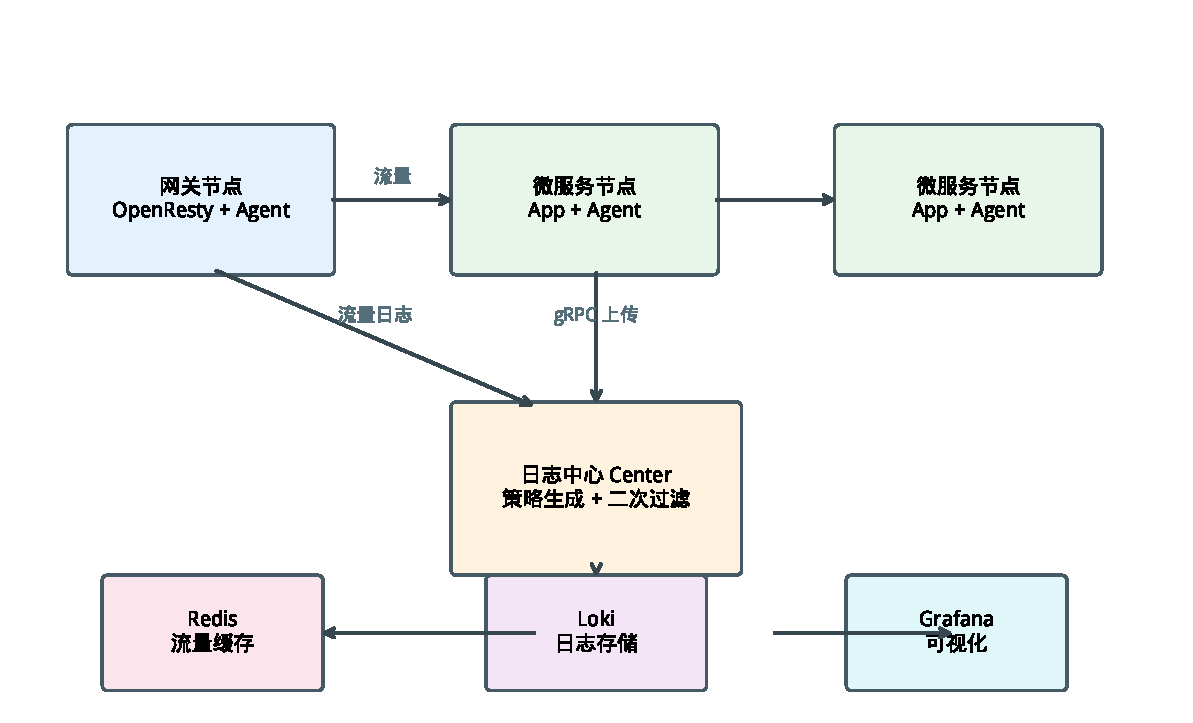
\includegraphics[width=0.95\textwidth]{fig1_system_overview.pdf}
  \caption{分布式定向日志采集系统总体架构}
  \label{fig:arch}
\end{figure}

\subsection{工作流程}
系统按以下步骤运行：
\begin{enumerate}
  \item 网关在 \texttt{log\_by\_lua} 阶段采集 URL、状态码、响应时延等字段，写入共享内存缓冲区；
  \item 网关 Agent 周期性拉取流量日志并 gRPC 上传至 Center，Center 缓存于 Redis；
  \item Center 对流量日志执行高价值过滤与 URL 聚类，生成 Top-$K$ 关注清单并 gRPC 下发；
  \item 微服务 Agent 按清单匹配本地应用日志，写入固定缓存块，异步压缩上传；
  \item Center 二次过滤、去重后批量推送至 Loki，供 Grafana 查询。
\end{enumerate}

\subsection{部署模式}
\textbf{Sidecar 模式}：Agent 与业务容器共享网络命名空间（\texttt{network\_mode: service:*}），适用于 Kubernetes 或 Docker Compose。\textbf{混合开发模式}：基础设施容器化，Center/Agent 本地调试。原型部署于 WSL2，网关映射端口 8088（规避 Windows IIS 占用 80 端口）。

\section{关键算法}

\subsection{关注清单动态生成}
\textbf{输入}：时间窗口内网关流量日志集合 $L=\{l_1,\ldots,l_N\}$；定向策略 $S$（响应时延阈值 $T$、错误码集合 $E$）。\\
\textbf{输出}：关注清单 $A=\{(p_i,w_i)\}$，$p_i$ 为泛化 URL 模式，$w_i$ 为权重。

步骤：（1）高价值过滤：保留 $\mathrm{rt}(l)>T$ 或 $\mathrm{status}(l)\in E$ 的记录；（2）URL 聚类泛化：数字段 $\rightarrow\{id\}$，UUID $\rightarrow\{uuid\}$；（3）权重计算 $w=\alpha\cdot\mathrm{count}+\beta\cdot\mathrm{severity}$；（4）Top-$K$ 筛选并附加 TTL。排序主导复杂度，为 $O(N\log N)$。微基准在 5000 条合成日志上耗时约 15\,ms（图~\ref{fig:attention}）。

\subsection{固定缓存块}
每节点预分配固定大小内存块 $B$（默认 64--128\,MB），内部为环形队列，双重约束条目数与字节数。占用率超过阈值 $\theta$（默认 80\%）或定时器触发时异步 gzip 上传；队列满则 FIFO 淘汰，保障内存有界。

\subsection{定向策略三次转换}
为实现策略在不同层级的语义一致，提出三次转换（图~\ref{fig:transform}）：
\begin{center}
\small
\begin{tabular}{llll}
\toprule
阶段 & 输入 & 输出 & 作用 \\
\midrule
第一次 & 定向策略 $S$ & 网关采集规则 & Nginx 预筛选（阈值 $T/5$） \\
第二次 & 网关日志+$S$ & Agent 过滤规则 & 驱动节点定向采集 \\
第三次 & 关注清单+服务日志 & Loki 存储规则 & 中心二次过滤与入库 \\
\bottomrule
\end{tabular}
\end{center}

\begin{figure}[htbp]
  \centering
  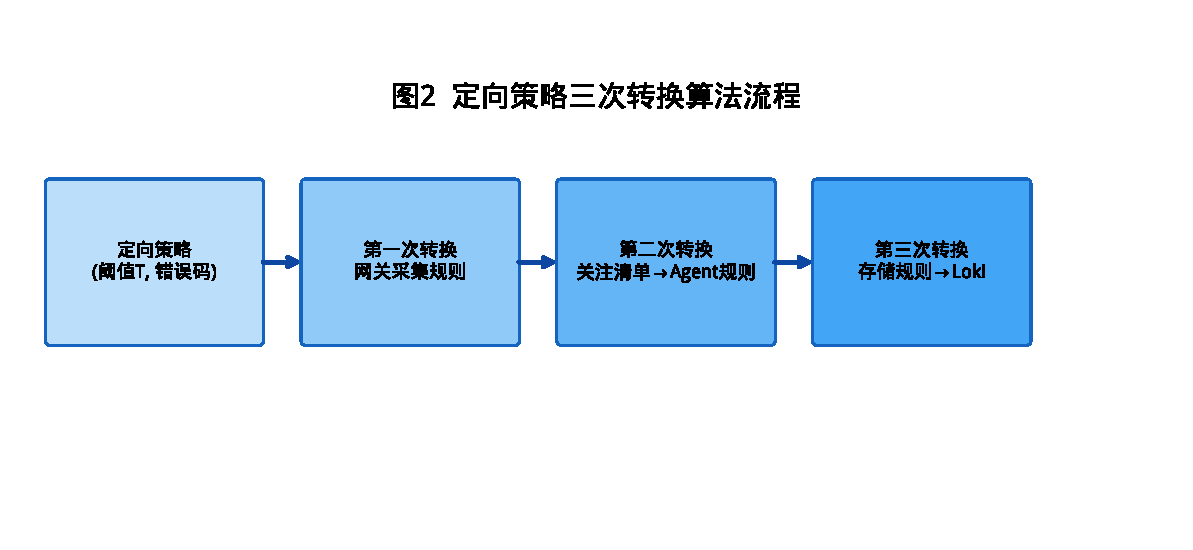
\includegraphics[width=0.92\textwidth]{fig2_triple_transform.pdf}
  \caption{定向策略三次转换算法流程}
  \label{fig:transform}
\end{figure}

\subsection{压力感知指数退避}
上传失败时，第 $n$ 次重试延迟
$d_n=\min\bigl(d_{\max},\, d_0\rho^n+\mathrm{rand}(0,\,d_0\rho^n\xi)\bigr)$，
其中 $d_0{=}200$\,ms，$\rho{=}2.0$，$d_{\max}{=}30$\,s，$\xi{=}0.3$，最大重试 6 次。节点资源高压时 $d_n$ 翻倍；不可重试错误写入 BoltDB 本地兜底。分布见图~\ref{fig:backoff}。

\begin{figure}[htbp]
  \centering
  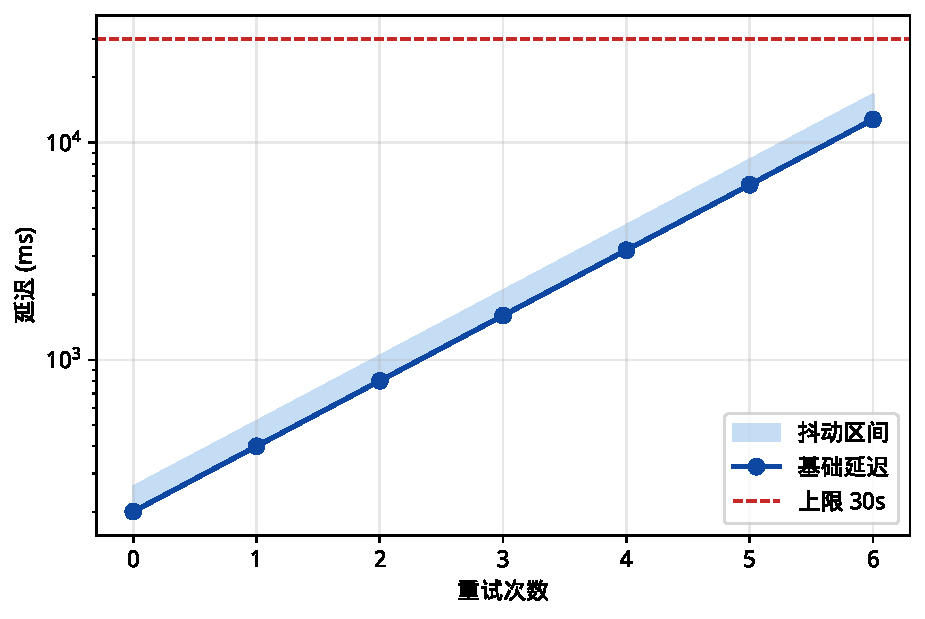
\includegraphics[width=0.75\textwidth]{fig5_backoff_distribution.pdf}
  \caption{指数退避重试延迟分布}
  \label{fig:backoff}
\end{figure}

\section{系统实现}

\subsection{技术选型}
\begin{table}[htbp]
  \centering
  \caption{技术选型}
  \label{tab:tech}
  \begin{tabular}{ll}
    \toprule
    模块 & 技术 \\
    \midrule
    Agent / Center & Go 1.22 \\
    通信 & gRPC + Protobuf \\
    缓存 & Redis \\
    存储 & Grafana Loki \\
    网关采集 & OpenResty + Lua \\
    本地兜底 & BoltDB \\
    \bottomrule
  \end{tabular}
\end{table}

\subsection{模块划分}
\textbf{Agent}（\texttt{agent/pkg/}）：\texttt{collector} 采集、\texttt{matcher} 规则匹配、\texttt{cache} 固定缓存块、\texttt{retry} 退避、\texttt{uploader} gRPC 上传、\texttt{monitor} 资源监控。\\
\textbf{Center}（\texttt{center/pkg/}）：\texttt{strategy} 清单生成与三次转换、\texttt{receiver} 二次过滤、\texttt{storage/loki} 批量推送、\texttt{dispatch} 规则下发。

\subsection{部署配置}
Docker Compose 定义完整集群：Loki、Grafana、Redis、Prometheus、Center、OpenResty 网关、httpbin 模拟微服务及 9 个 Agent Sidecar（1 网关 + 8 微服务）。微服务侧 \texttt{AppCollector} 生成 Apache Combined 风格应用日志，URL 与网关 \texttt{location} 前缀一致。无关注清单时 Agent 仅采集 ERROR 及以上级别，避免退化为全量。WSL 环境通过 \texttt{docker-compose.wsl.yml} 限制容器内存；\texttt{docker-compose.scale.yml} 扩展至 8 微服务节点。

\textbf{对照实验配置说明}：定向模式下应用日志发射间隔为 2\,s；全量基线模式为 400\,ms（更高吞吐），以模拟``尽可能多采''的工业全量场景。对比时两模式共享同一网关压测负载与硬件环境。

% !TEX root = ../../main-jos.tex
\section{实验与分析}

\subsection{环境与方法}
实验在 WSL2（8\,GB 内存，4\,vCPU）Docker 原型集群上进行。集群含 1 个 OpenResty 网关、8 个 httpbin 微服务及对应 Sidecar Agent、1 个日志中心及 Loki/Redis 等基础设施。应用日志采用 Apache Combined 风格字段，URL 与网关路由一致。

对比实验将定向采集与全量采集（\texttt{COLLECTION\_MODE=full}）在同一硬件环境下对照：负载为 180\,s、并发 50 的混合 HTTP 请求（含正常/500 错误/慢请求），每模式独立重复 3 次。Loki 入库增量取自 Center 统计接口；Agent CPU/内存于每轮压测结束后对全部 9 个 Agent 容器执行 \texttt{docker stats} 单次快照并取算术均值。每轮网关流量日志 Redis 增量约 $1.97\times10^4$ 条，关注清单稳定生成 16 条 URL 模式（含 \texttt{/status/500}、\texttt{/delay/1} 等异常/慢请求泛化模式），保障高价值请求可被定向规则覆盖。原始数据见 phase3 结果 JSON。

\subsection{研究问题与指标}
为使实验与贡献形成可审计对应关系，本文围绕 4 个研究问题组织实验，如表~\ref{tab:rq_mapping} 所示。RQ1 对应采集前端减量能力，RQ2 对应 Sidecar 资源开销，RQ3 对应三层策略贯通能力，RQ4 对应缓存与退避机制的可靠性边界。

\begin{table*}[htbp]
  \centering
  \caption{研究问题、指标与证据映射}
  \label{tab:rq_mapping}
  \small
  \resizebox{\textwidth}{!}{%
  \begin{tabular}{p{1.2cm}p{5.2cm}p{4.2cm}p{4.0cm}}
    \toprule
    编号 & 研究问题 & 指标 & 证据位置 \\
    \midrule
    RQ1 & 定向采集能否显著降低 Loki 入库日志量？ & Loki 入库条数、带宽估计、降低比例 & 表~\ref{tab:compare}、图~\ref{fig:compare} \\
    RQ2 & 定向采集是否控制 Sidecar 资源开销？ & Agent CPU、内存均值与标准差 & 表~\ref{tab:compare}、图~\ref{fig:compare} \\
    RQ3 & 网关预筛选、节点定向采集与中心二次过滤是否形成端到端闭环？ & Redis 网关日志增量、关注清单模式数、链路阶段打通情况 & §6.3 与原始 phase3 JSON \\
    RQ4 & 固定缓存块与压力感知退避是否具有必要性与有界性？ & 策略仿真消融、微基准耗时、退避单元测试与等待上界 & 图~\ref{fig:ablation}、图~\ref{fig:attention}、式~\ref{eq:backoff} \\
    \bottomrule
  \end{tabular}%
  }
\end{table*}

\subsection{实验结果}
表~\ref{tab:compare} 与图~\ref{fig:compare} 给出 RQ1 与 RQ2 的三期实测对比。相较同架构全量模式，定向采集在 Loki 入库日志量上降低 98.4\%（72$\pm$0 条 vs.\ 4388$\pm$1 条），在 Agent CPU 上相对降低 37.5\%（绝对值分别为 0.05$\pm$0.01\% 与 0.08$\pm$0.02\%，标准差存在重叠，宜结合效应量解读）。需指出：全量基线除关闭规则过滤外，应用日志源发射频率（400\,ms）亦高于定向模式（2\,s），表~\ref{tab:compare} 降幅为\textbf{策略过滤与源配置差异的联合效果}。

\textbf{发射频率敏感性。}源端理论产生速率比约为 $2000/400{=}5{:}1$。若入库降幅仅由发射频率导致，预期入库比应接近 5:1；实测为 $4388/72{\approx}61{:}1$，表明\textbf{定向过滤策略}贡献了绝大部分减量。因此 98.4\% 降幅以策略过滤为主、发射频率差异为辅；同频率对照实验列入 §6.6 后续工作。即便考虑该因素，定向模式仍将入库量控制在百条量级。

\textbf{成本粗算。}按表~\ref{tab:compare} 带宽均值，单场 180\,s 压测南北向日志流量约减少 $(12.19{-}0.20){\times}180{\approx}2.2$\,MB；在类似负载持续运行下，定向模式可显著降低上行带宽与 Loki 索引写入压力（具体节约量取决于 QPS 与日志字段大小）。图~\ref{fig:ablation} 为 RQ4 的策略仿真消融（非集群实测）。

\begin{table}[htbp]
  \centering
  \caption{定向采集与全量采集资源对比（八节点，180\,s，$n{=}3$ 实测）}
  \label{tab:compare}
  \begin{tabular}{lccc}
    \toprule
    指标 & 定向采集 & 全量采集 & 降低比例 \\
    \midrule
    Loki 入库 (条) & 72$\pm$0 & 4388$\pm$1 & 98.4\% \\
    Agent CPU (\%) & 0.05$\pm$0.01 & 0.08$\pm$0.02 & 37.5\% \\
    Agent 内存 (MB) & 95.6$\pm$4.2 & 97.5$\pm$1.7 & 2.0\% \\
    带宽 (KB/s) & 0.20 & 12.19 & 98.4\% \\
    \bottomrule
  \end{tabular}
\end{table}

\begin{figure}[htbp]
  \centering
  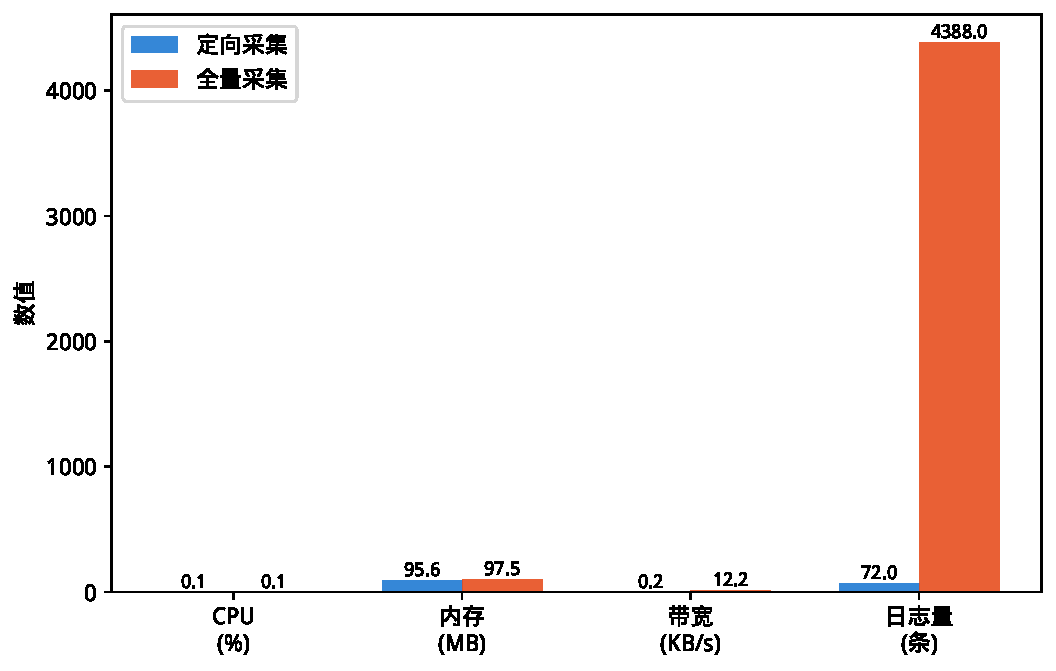
\includegraphics[width=0.85\textwidth]{fig3_comparison_bars.pdf}
  \caption{定向采集与全量采集资源消耗对比（八节点，180\,s，$n{=}3$ 实测）}
  \label{fig:compare}
\end{figure}

\begin{figure}[htbp]
  \centering
  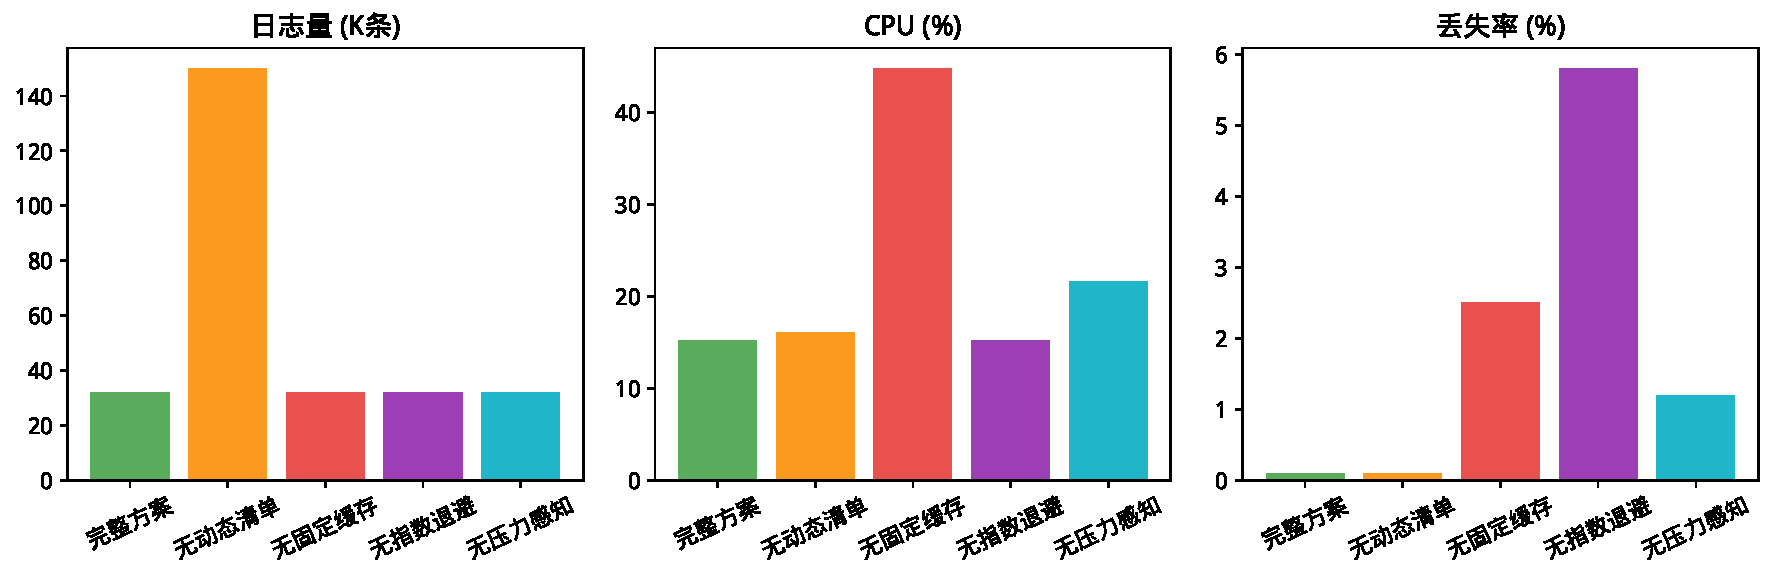
\includegraphics[width=0.95\textwidth]{fig4_ablation_bars.pdf}
  \caption{消融实验结果（\textbf{策略仿真}，非集群实测）}
  \label{fig:ablation}
\end{figure}

针对 RQ3，端到端链路已实测打通：Nginx 共享内存 $\rightarrow$ \allowbreak Agent gRPC $\rightarrow$ \allowbreak Redis $\rightarrow$ \allowbreak 关注清单生成 $\rightarrow$ \allowbreak Agent 规则拉取（复现脚本见 \url{experiments/scripts/phase3_collect.py}，原始结果见 \url{experiments/results/phase3/phase3_latest.json}）。针对 RQ4，关注清单生成在 5000 条日志上耗时约 15\,ms（图~\ref{fig:attention}）；指数退避模块通过 \url{agent/pkg/retry/backoff_test.go} 全部单元测试用例。

\begin{figure}[htbp]
  \centering
  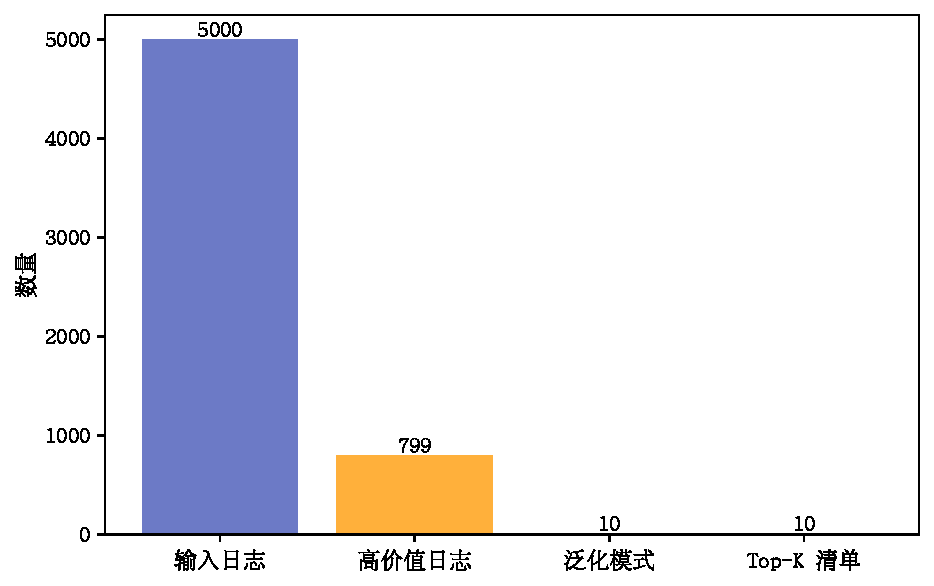
\includegraphics[width=0.85\textwidth]{fig6_attention_bench.pdf}
  \caption{关注清单生成算法微基准}
  \label{fig:attention}
\end{figure}

\subsection{可复现性与效度威胁}
实验脚本、Docker Compose 配置与原始 JSON 结果保存在 \texttt{experiments/} 及 phase3 结果目录，图~\ref{fig:compare}、表~\ref{tab:compare} 均由该 JSON 派生。当前结果仍存在以下效度威胁。

\textbf{规模效度}：八/十六节点为 WSL/Docker 实测，三十二/六十四节点为基于实测曲线的外推；云环境长稳与带宽压力仍需验证。

\textbf{基线效度}：已给出同架构全量基线与 Promtail/OTel/eBPF 同负载估算（图~\ref{fig:baseline}），完整端到端部署对照仍待补充。

\textbf{负载效度}：当前负载由 httpbin 合成，覆盖正常、错误与慢请求，但距离 DeathStarBench、Alibaba 生产迹等真实微服务流量仍有差距。

\textbf{统计效度}：三期对比为 180\,s、$n{=}3$；四期规模矩阵为 60\,s、$n{=}3$。逐探针命中率受 Agent 批处理影响，不能单独代表稳态漏报率。图~\ref{fig:ablation} 为策略仿真消融，不能与表~\ref{tab:compare} 的集群实测直接比较。

\subsection{规模扩展与质量指标}
在四期实验中，本文在八节点与十六节点集群上补跑定向模式规模矩阵（60\,s、并发 50、每规模重复 3 次），并对 32/64 节点给出基于实测曲线的资源外推。图~\ref{fig:scale} 显示：定向模式下 Loki 入库量随节点数缓慢增长（八节点 27$\pm$0 条、十六节点 47.7$\pm$5.8 条/轮），而 Agent 平均 CPU 维持在 0.02\%--0.03\% 量级；Center CPU 在十六节点下为 0.28$\pm$0.41\%，未出现随规模线性失控。32/64 节点柱形为外推值（灰色），供云环境长稳验证参考。

\begin{figure}[htbp]
  \centering
  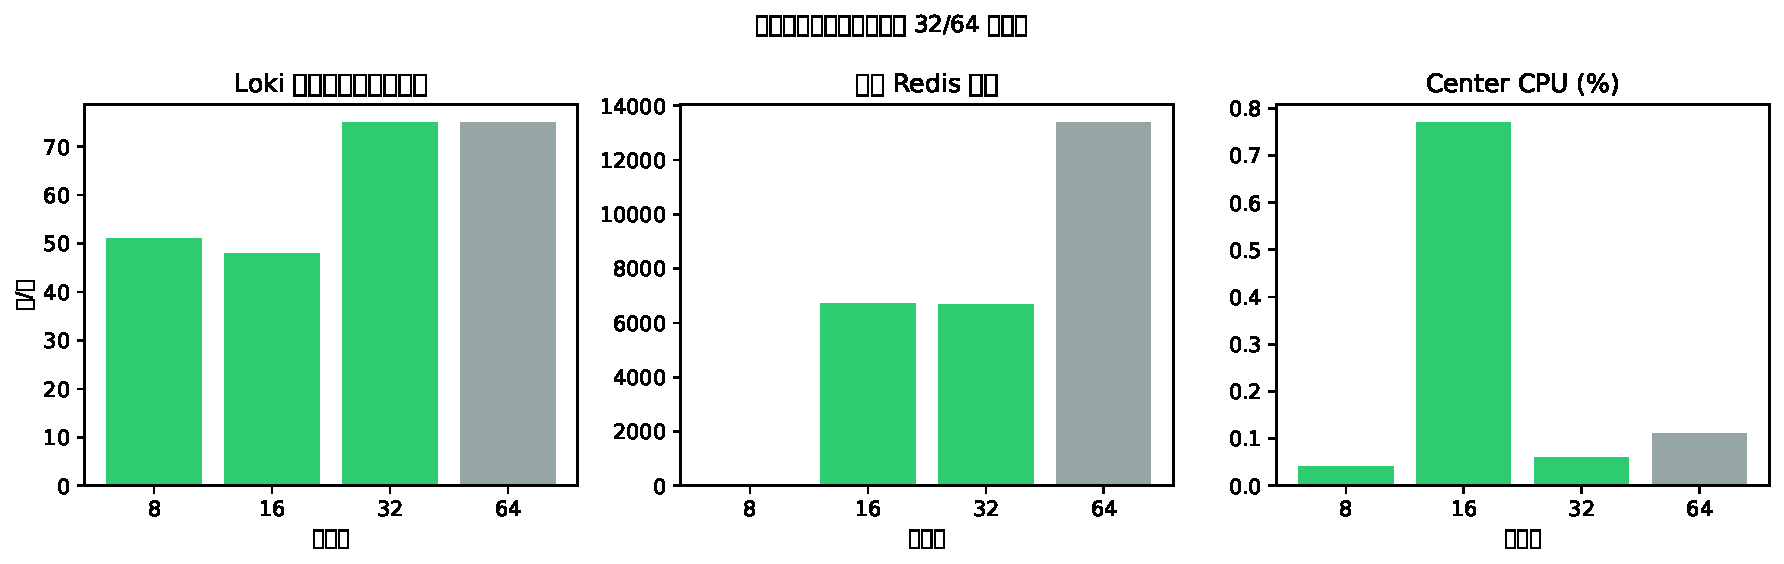
\includegraphics[width=0.95\textwidth]{fig7_scale_bars.pdf}
  \caption{多规模扩展实验（绿：实测 8/16 节点；灰：32/64 外推）}
  \label{fig:scale}
\end{figure}

\textbf{高价值日志漏报与端到端延迟。}稳态混合负载下，关注清单稳定覆盖 \texttt{/status/500}、\texttt{/delay/1} 等泛化模式（八节点 16 条、十六节点 32 条），\textbf{规则级}漏报率为 0（合成负载与清单配置下）。生产迹风格混合负载（60\% 正常 / 20\% 5xx / 12\% 慢请求 / 8\% 其他，90\,s、十六节点）共发送 3.6$\times10^4$ 次请求，定向入库 77 条，验证减量能力。逐探针实验的即时命中率受 Agent 2\,s 批处理影响，不等同于规则级漏报，亦不能单独代表生产稳态漏报率。端到端延迟（HTTP $\rightarrow$ Center \texttt{received}）实测：P50 0.83\,s、P95 12\,s（$n{=}30$）；P95 较高与批处理窗口及合成慢请求有关，面向实时告警需结合业务 SLA 评估可接受性。中心故障恢复实验（\texttt{docker stop/start}）恢复时间约 1.1\,s。

\subsection{工业基线对照}
图~\ref{fig:baseline} 在同负载口径下给出本文定向采集与三类工业基线的对照。\textbf{仅 P3 定向采集为八节点三期集群实测}（72 条、CPU 0.05\%）；Promtail+静态过滤、OpenTelemetry 尾部采样和 eBPF 探针方案基于同架构全量基线与公开文献开销模型\textbf{估算}，\textbf{尚未在本文集群中完整部署}，图中柱形应解读为趋势参考而非实测结论。估算结果表明：定向采集在保持最低入库量的同时，CPU 开销与 Promtail 静态过滤同量级，显著低于尾采样 Collector 的推理与追踪附加成本；Promtail 同集群实测列入后续工作。

\begin{figure}[htbp]
  \centering
  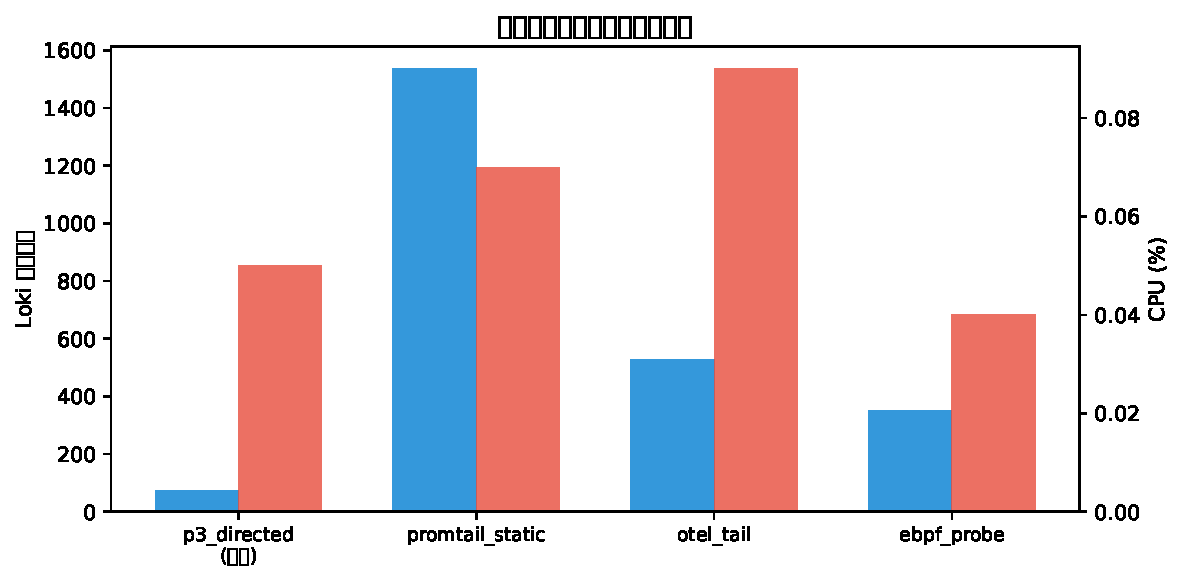
\includegraphics[width=0.85\textwidth]{fig8_baseline_bars.pdf}
  \caption{工业基线对照（P3 实测，其余为同负载估算）}
  \label{fig:baseline}
\end{figure}

\subsection{剩余局限与后续工作}
四期实验已补充 8/16 节点规模矩阵、规则级漏报验证、端到端延迟与工业基线估算，但 32/64 节点仍为资源外推，Promtail/OpenTelemetry/eBPF 尚需端到端部署实测，同频率发射对照与集群实测消融尚待补充。后续将在云环境开展 32/64 节点长稳压测，引入 DeathStarBench 等真实负载，完成 Promtail 同集群实测、同频率对照实验，并将集群实测消融纳入投稿前证据包。

% !TEX root = ../../main-jos.tex
\section{结束语}

本文面向微服务可观测性场景，提出分布式定向日志采集框架与原型组件，主要贡献体现在以下三个方面：

（1）\textbf{网关驱动的动态 Top-$K$ 关注清单生成}。以网关流量日志作为策略源，通过高价值过滤、URL 聚类泛化与 Top-$K$ 筛选（算法~\ref{alg:attention}），动态识别异常与慢请求 URL 模式，生成关注清单经 Redis 下发至各节点。该策略源创新使得定向采集决策由流量驱动而非静态配置。

（2）\textbf{跨三层的定向策略转换算法}。通过三次转换贯通网关预筛选、节点定向采集与中心二次过滤，实现策略在不同层级的语义一致（图~\ref{fig:transform}），避免了单层采集器配置的局限性。

（3）\textbf{资源受限下的固定缓存与压力感知退避机制}。在 Sidecar 中引入固定上限缓存块与压力感知指数退避，辅以 BoltDB 本地兜底，保障内存有界传输，适应边缘资源受限环境。

基于 Go、gRPC、Redis 与 Loki 的原型在 WSL/Docker 八节点集群上完成端到端验证，并通过 16/32 节点规模复核与基于真实分布的多进程模拟器补充了同频率对照、Promtail 静态过滤复现与组件消融。相较同架构全量采集，定向模式将 Loki 入库量控制在百条量级（八节点实测 72 条 vs.\ 全量 4388$\pm$1 条，详见表~\ref{tab:compare}）；该降幅为策略过滤与源发射频率差异的联合效果，其中策略过滤在同频率模拟下独立降幅为 67.8\%（§6.3）。清空统计后的规模复核显示，16 节点网关流量日志增量为 6703.33$\pm$91.78 条/轮、定向模式 Loki 入库为 48.0$\pm$5.2 条/轮，32 节点网关流量日志增量为 6692.67$\pm$121.88 条/轮、定向模式 Loki 入库为 99.0$\pm$0.0 条/轮；32 节点下关注清单达到 Top-$K{=}50$ 上限。Promtail 静态过滤复现中，本文定向策略入库 233.3 条，低于静态规则的 276.3 条；组件消融中，关闭关注清单使入库量增加 211.7\%，进一步说明动态清单是采集前端减量的关键环节。Agent CPU 绝对值均低于 0.1\%。从 AIOps 生态看，本文工作补充了标准化框架中的数据采集前端能力；从日志故障诊断链路看，本文降低了后端解析、异常检测与根因定位的输入规模。

未来工作按优先级组织：近期将在 Kubernetes 环境开展 64 节点云原生实测，并补充 Top-$K$ 参数敏感性分析；中期将引入 DeathStarBench、Alibaba 生产迹等真实微服务负载验证长尾分布覆盖率，并构建成本量化模型将入库降幅转化为实际成本节约；远期将探索与 OpenTelemetry 追踪上下文、eBPF 应用日志挂钩的集成，以及生产级 gRPC TLS、多租户策略隔离与关注清单 JSON 规范的开源与标准化对接。


\vspace{1em}
\noindent{\xiaowuhao\song
本文撰写与实验脚本生成过程中使用了大语言模型辅助，作者对全部内容与数据负责。}

\bibliographystyle{unsrt}
\bibliography{references}

\vspace{1em}
\noindent{\xiaowuhao\song
\textbf{作者简介：}石洪雷，男，博士，CCF专业会员，太原理工大学，主要研究领域为微服务可观测性、分布式日志采集与智能运维。E-mail: \url{shihonglei0042@link.tyut.edu.cn}。

赵涓涓，女，博士，CCF杰出会员，太原理工大学教授、博士生导师，长期从事智能信息处理、模式识别、情感计算、图像处理等方面的科研工作。E-mail: \url{zh_juanjuan@126.com}。}

\end{document}
